\label{sec:pac}

\rnote{For this section, you should first define PAC-Bayes bound and explain the role of prior and posterior. Then you should say what posterior \cite{dziugaite2017computing} optimize over and explain how our posterior is different. After that skip all the details about calculation and directly show the results (the table, the figures might also belong to appendix). This shouldn't be a very long section.}

\subsection{Methods}
\cnote{We need to briefly explain the PAC-Bayes bound in \citet{dziugaite2017computing}, e.g., what is SNN, what does the bound look like, what's prior/posterior.}
Our layer-wise Hessian approximation can be used to efficiently improve the computing of nonvacuous PAC-Bayes generalization bounds presented in \citet{dziugaite2017computing}.\ynote{Should we cite in () or in the sentence?}\cnote{In the sentence.} The core part of their algorithm is to model the posterior as a multivariate normal distribution $\N(\vw, \diag(\vs))$ and optimizing $\vw$ and $\vs$. Intuitively, the optimization of $\vs$ is to search for an optimal deviation of each parameter that can balance the the training error and the KL divergence between prior and posterior. Since the covariance matrix is diagonal, the search is along the direction of each standard basis. In general, the variance should be larger for a flatter direction and smaller for a sharper direction. However, directions of the standard basis may not be the optimal direction for the search. If we consider the loss landscape close to the minimum, sharper directions correspond to the Hessian's eigenvectors of lareger eigenvalues. \ynote{Cite or put some description in the Preliminary?} Thus, it may be a good idea to perform the search using the basis of Hessian's eigenvectors.

Since we can only use standard basis to calculate training loss, a change of basis is required. A direct change of basis using eigenvectors of Hessian is computationally prohbitive.\ynote{except for very small networks.} However, efficient approximate change of basis can be performed using the Kronecker factorized layer-wise Hessians. Let $\mU$ be the full eigenspace of $\E[\mM]$ and $\mV$ be that of $\E[\vx\vx^T]$ with eigenvectors as columns. We define $\Mat$ as the reshape of a vector to the shape of the parameter matrix $\mW$ of that layer. Then, let $\vv$ be the vector in standard basis. We have the new vector $\vv'$ in Hessian basis as
\begin{equation}
    \vv' = \vect\left[\mU^T\Mat(\vv)\mV\right].
\end{equation}
The calculation is thus much faster and a reverse process can be easily applied to change a vector back to the standard basis.\ynote{Should we omit the entire calculation? Or just say implicit matrix multiplication and refer to Appendix} This algorithm is called Approx Hessian.

In addition, since the posterior mean $\vw$ changes during the optimization, it is reasonable to use eigenvectors of the Hessian with respect to the current $\vw$. This algorithm is called Iterative Hessian, where we calculate new eigenvectors every several epochs.\ynote{We should results where we calculate new eigenvectors every 10 epochs but also tried other settings. Should we specify 10 here?}

\subsection{Results}
We used identical dataset, network structures and experiment settings as in \citet{dziugaite2017computing}, with a few adjustments in hyperparameters. We also adding FC2 we used in \cref{sec:hessian}. T-$600_{10}$ and FC$2_{10}$ are trained on standard MNIST while all others are trained on 2-class MNIST. The results are shown in \cref{tab:pac}. The network are expressed as X-$n^m$, indicating $m$ hidden layers with $n$ nodes each, trained on true labels (X=T) or random labels (X=R).\ynote{The generalization gap shown is our generalization gap, which is similar to the previous work.}

\begin{table}[th]
\caption{Optimized PAC-Bayes bound with Hessian Information \znote{need change}}

\begin{center}
\begin{tabular}{lccccccc}
\multicolumn{1}{c}{\bf Experiments}  & T-$600$ & T-$1200$ & T-$300^2$ & T-$600^2$ & R-$600$ & T-$600_{10}$ & FC$2_{10}$
\\ \hline \\
Generalization gap      & 0.0153  & 0.0161  & 0.0150 & 0.0148  & 0.4925 & 0.0180 & 0.0208 \\
Vanilla*                 & 0.1540  & 0.1754 &  0.1686 & 0.1921  & 0.6046  & 0.2879 & 0.4165 \\
Approx Hessian          & 0.1464 & 0.1726  & 0.1417  & 0.1712  & \textbf{0.5653} & 0.2424 & 0.2725 \\
Iterative Hessian       &  \textbf{0.1198}  & \textbf{0.1417}  & \textbf{0.1249}  & \textbf{0.1456}  & 0.5681 & \textbf{0.2132}   & \textbf{0.2145}  \\
\end{tabular}
\end{center}
\label{tab:pac}
\end{table}
\ynote{Iterative Hessian for FC2 is still runing. Previous results have some hyperparameter issues.}

Compared with previous work and vanilla algorithm, we can see a significant decrease of PAC-Bayes bound using Approximated Hessian algorithm and a further decrease using Iterative Hessian algorithm. Bounds for standard MNIST are not as good but still nonvacuous.

We also plotted the natural logarithm of final variance, $\vs$. The Figure 5.1 shown below is for (Approx Hessian of T-600) \znote{FC2}. The basis is ordered with decreasing eigenvalues. We can see that direction associated with larger eigenvalue has a smaller variance. This agrees with our presumption that top eigenvectors are aligned with sharper directions and should have smaller variance after optimization.

\begin{figure}[ht]
    \centering
    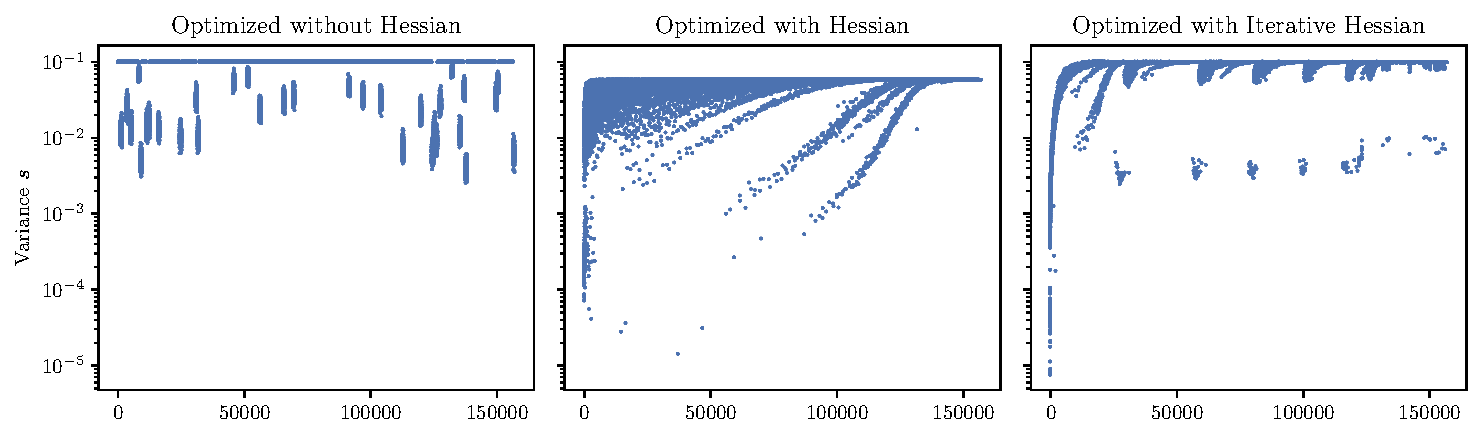
\includegraphics[width=\textwidth]{Figures/PacBayes/FC2_10cls/sigma_post_compare_iter_Sigma_post_MNIST_Exp1FC2_fixlr0.01_fc1.weight.pdf}
    \captionsetup{justification=centering}
    \caption{Variance of optimized posterior. (first hidden layer of FC2, trained on MNIST)}
    \label{fig:PAC}
\end{figure}

Detailed algorithms and experiment settings are in \cref{sec:appendix_pac}.